% !TEX TS-program = XeLaTeX
\documentclass[11pt, oneside,american]{book}   	
\usepackage[margin=1in]{geometry}                		% See geometry.pdf to learn the layout options. There are lots.
\geometry{letterpaper}                   		% ... or a4paper or a5paper or ... 
\usepackage{graphicx}
\usepackage{float}
\usepackage{wrapfig}
\usepackage[american]{babel}
\usepackage[babel]{csquotes}
\usepackage{etoolbox,xkeyval,ifthen,url}
\usepackage{enumitem}
\usepackage[
	backend=biber,
	annotation,
	loadfiles=true % this forces load of external annotations - based on naming convention
]{biblatex-chicago}
\usepackage{filecontents}
\usepackage[all]{nowidow}
\usepackage{titlesec}
\newcommand{\sectionbreak}{\clearpage}
\usepackage{hyperref}
\input{insbox}
\makeatletter
\@InsertBoxMargin = 10pt
\makeatother

\addbibresource{bibs-no-anno/bcarlier.bib}
\addbibresource{bibs-no-anno/gdobbs.bib}
\addbibresource{bibs-no-anno/iglazer.bib}
\addbibresource{bibs-no-anno/shaq.bib}
\addbibresource{bibs-no-anno/ahindle.bib}
\addbibresource{bibs-no-anno/shutchinson.bib}
\addbibresource{bibs-no-anno/r2h2.bib}
\addbibresource{bibs-no-anno/akoot.bib}
\addbibresource{bibs-no-anno/cscholefield.bib}
\addbibresource{bibs-no-anno/ssquire.bib}
\addbibresource{bibs-no-anno/gwilliamson.bib}


%the following removes the dot between the entries when \\ occurs after annotation
% the \\ is there to ensure space between the annotations from >1 contributor
% and its hard to avoid on the last line, thus this command
\renewcommand*{\finentrypunct}{}%

% the following adjusts the biblatex-chicago macros to provide a hyperlink on the citations
\DeclareFieldFormat{citehyperref}{%
\DeclareFieldAlias{bibhyperref}{noformat}% Avoid nested links
\bibhyperref{#1}}

\savebibmacro{cite}

\renewbibmacro*{cite}{%
  \printtext[citehyperref]{%
  \restorebibmacro{cite}%
  \usebibmacro{cite}}}
% end of hyperlink patch

%SetFonts
\usepackage{fontspec}
% separate in order to make it easier to maintain and try others

% select one:
%\setmainfont{American Typewriter} % 
%\setmainfont{Big Caslon Medium} % 
\setmainfont{Noto Sans Regular} % 


% select one:
%\setsansfont[Scale=MatchLowercase]{Gill Sans} % 
%\setsansfont[Scale=MatchLowercase]{Helvetica Neue Thin} % 
\setsansfont[Scale=MatchLowercase]{Noto Sans Italic} % 


%\setmonofont[Scale=MatchLowercase]{Monaco}
\setmonofont[Scale=MatchLowercase]{Noto Mono} 
 
\providecommand{\tightlist}{%
  \setlength{\itemsep}{0pt}\setlength{\parskip}{0pt}}

\setcounter{secnumdepth}{-1}

\setlist{nosep} %tighten up lists

\begin{document}
\frontmatter
\begin{titlepage}
	\centering
	{\scshape\huge\bfseries  Identity Professionals Recommend \par}
	\vspace{1cm}
	{\scshape\LARGE An annotated bibliography\par}
	\vspace{1.5cm}
	{\large Updated and Issued from Time to Time\par}
	\vspace{2cm}
	{\Large\itshape\bfseries Contributions by the membership of IDPro\par}
	\vfill
	compiled by\par
	\textsc{The Body of Knowledge Committee}
	\vfill
% Bottom of the page
	{\large \today\par}
	\vfill
	\includegraphics[width=0.20\textwidth]{media/idpro-logo.png}\par\vspace{1cm}
	\clearpage
\end{titlepage}
% include this file in the main .tex file
\section{Disclaimer}

While the content in this bibliography is reviewed by the Body of Knowledge Committee, IDPro cannot provide any guarantee that the material included is correct or applicable in all situations, or that it is freely available to the public.

\pagenumbering{gobble} 
\vspace*{6in}
\char"00A9 IDPro, Inc., 2019
\clearpage
\pagenumbering{roman} 

\section{Preface}

Beginnings aren’t simple; they take courage and curiosity. Courage to try something new is applauded, whether what is new is a new profession, such as  identity management, or a new discipline, such as learning federation after already mastering access certification. Regardless, setting out to do something new requires the curiosity to figure out how to do it.

A consistent challenge in our profession is finding the resources from which to learn that new thing. IDPro’s mission is to help do just that: connecting professionals to learn from one another, providing opportunities to learn from experts, and building resources from which professionals can learn. And this bibliography is one such resource.

The collation of suggestions from identity professionals, this bibliography hopes to provide a needed resource for people with the courage and curiosity to begin something. The books, blogs, and articles referenced within span a wide range of topics and a wide range of approaches. And more that than, it offers a glimpse as to why your peers suggested the resource in the first. Knowing why someone read something is a useful clue as to the value you’ll get from reading the same thing.

This bibliography represents a beginning in and of itself. It is the first, of what will be many resources, that our Body of Knowledge Committee has created. I applaud the group for their courage and curiosity to begin and hope you find a gem or two in here that helps you on your beginning!

\vspace{24pt}
{\setlength{\parindent}{0cm}
\textsc{
January 10, 2019\\
Ian Glazer\\
Founder and President, IDPro}
}

\section{Introduction}
This document is intended as an a way to convey some of the accumulated wisdom and knowledge of the members of IDPro. 
It is in the form of an annotated bibliography, where the references may be books or any other form of knowledge transfer.  At the same time, this document is a way for individual members of IDPro to highlight their experience and expertise.  It is not intended to be a marketplace.  Rather it is a way to extend the benefits of community to the members of IDPro.

All members of IDPro are encouraged to make contributions.  And contributions of content are appreciated. The contributors' biographic details,  likenesses and annotations are subject to only to light editing by the Body of Knowledge Committee.  The contributors are encouraged to submit annotations that are fresh and friendly and fun. You may find some of them contain a degree of humor not normally associated with something as dry as knowledge transfer.

Please contact @bok for the best method to contribute.

\vspace{24pt}
{\setlength{\parindent}{0cm}
\textsc{
January 20, 2019\\
George Dobbs\\
Chair, Body of Knowledge Committee, IDPro}
}

\mainmatter
\section{The Contributors}
\subsection{Bertrand~Carlier} \textsf{Paris, France} \par \setlength{\columnsep}{0pt} \begin{wrapfigure}{l}{0.25\textwidth} \centering 
\includegraphics[width=0.18\textwidth]{bios/bcarlier.jpg} \end{wrapfigure} \input{bios/bcarlier.txt} \subsubsection{Recommendations}\begin{enumerate}
\item \cite{Bertocci2019}
\item \cite{Siriwardena2016}
\end{enumerate}\noindent\rule{\textwidth}{0.2pt}

\subsection{George~Dobbs} \textsf{Hartford, Connecticut, USA area} \par \setlength{\columnsep}{0pt} \begin{wrapfigure}{l}{0.25\textwidth} \centering \includegraphics[width=0.18\textwidth]{bios/gdobbs.png} \end{wrapfigure} \input{bios/gdobbs.txt} \subsubsection{Recommendations}\begin{enumerate}
\item \cite{Cameron2005}
\item \cite{Hoffman1977}
\end{enumerate}\noindent\rule{\textwidth}{0.2pt}

\subsection{Ian~Glazer} \textsf{Washington, DC, USA} \par \setlength{\columnsep}{0pt} \begin{wrapfigure}{l}{0.25\textwidth} \centering 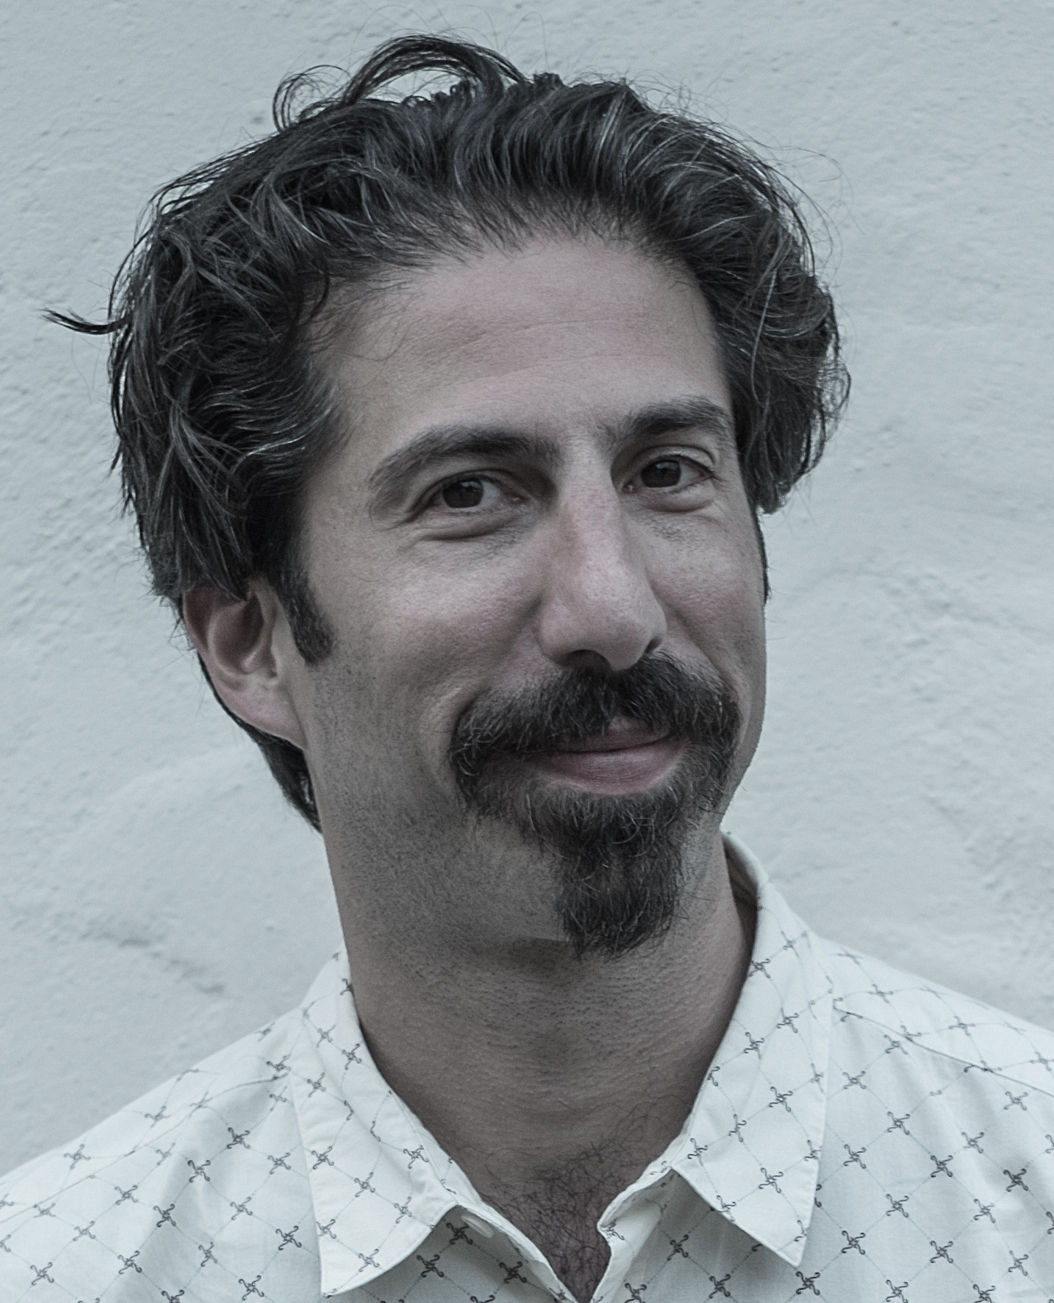
\includegraphics[width=0.18\textwidth]{bios/iglazer.jpg} \end{wrapfigure} \input{bios/iglazer.txt} \subsubsection{Recommendations}\begin{enumerate}
\item \cite{Clippinger2007}
\item \cite{Richer2017}
\end{enumerate}\noindent\rule{\textwidth}{0.2pt}

\subsection{Salman (Shaq)~Haq} \textsf{Mclean, Virgina, USA area} \par \setlength{\columnsep}{0pt} \begin{wrapfigure}{l}{0.25\textwidth} \centering \includegraphics[width=0.18\textwidth]{bios/shaq.jpg} \end{wrapfigure} \input{bios/shaq.txt} \subsubsection{Recommendations}\begin{enumerate}
\item \cite{Windley2005}
\end{enumerate}\noindent\rule{\textwidth}{0.2pt}

\subsection{Andi~Hindle} \textsf{Oxfordshire, UK} \par \setlength{\columnsep}{0pt} \begin{wrapfigure}{l}{0.25\textwidth} \centering 
\includegraphics[width=0.18\textwidth]{bios/ahindle.jpg} \end{wrapfigure} \input{bios/ahindle.txt} \subsubsection{Recommendations}\begin{enumerate}
\item \cite{Carlier2018}
\item \cite{Moore1991}
\end{enumerate}\noindent\rule{\textwidth}{0.2pt}

\subsection{Steve~Hutchinson} \textsf{Richmond, Virginia, USA area} \par \setlength{\columnsep}{0pt} \begin{wrapfigure}{l}{0.25\textwidth} \centering \includegraphics[width=0.18\textwidth]{bios/shutchinson.jpg} \end{wrapfigure} \input{bios/shutchinson.txt} \subsubsection{Recommendations}\begin{enumerate}
\item \cite{Birch2014}
\item \cite{Hardjono2016}
\item \cite{Nayyar2018}
\item \cite{Richer2017}
\item \cite{Schwartz2018}
\end{enumerate}\noindent\rule{\textwidth}{0.2pt}

\subsection{Rainer~Hörbe} \textsf{Vienna, Austria} \par \setlength{\columnsep}{0pt} \begin{wrapfigure}{l}{0.25\textwidth} \centering 
\includegraphics[width=0.18\textwidth]{bios/r2h2.jpg} \end{wrapfigure} \input{bios/r2h2.txt} \subsubsection{Recommendations}\begin{enumerate}
\item \cite{IAMPrimer2016}
\end{enumerate}\noindent\rule{\textwidth}{0.2pt}

\subsection{André~Koot} \textsf{Amsterdam, Netherlands area} \par \setlength{\columnsep}{0pt} \begin{wrapfigure}{l}{0.25\textwidth} \centering \includegraphics[width=0.18\textwidth]{bios/akoot.jpg} \end{wrapfigure} \input{bios/akoot.txt} \subsubsection{Recommendations}\begin{enumerate}
\item \cite{Cameron2005}
\item \cite{Hardt2005}
\item \cite{Harper2006}
\item \cite{Williamson2017}
\end{enumerate}\noindent\rule{\textwidth}{0.2pt}

\subsection{Corey~Scholefield} \textsf{Victoria, British Columbia, Canada area} \par \setlength{\columnsep}{0pt} \begin{wrapfigure}{l}{0.25\textwidth} \centering \includegraphics[width=0.18\textwidth]{bios/cscholefield.jpg} \end{wrapfigure} \input{bios/cscholefield.txt} \subsubsection{Recommendations}\begin{enumerate}
\item \cite{Hazelton2015}
\item \cite{Prasad2012}
\item \cite{Windley2005}
\end{enumerate}\noindent\rule{\textwidth}{0.2pt}

\subsection{Sarah~Squire} \textsf{Seattle, Washington, USA area} \par \setlength{\columnsep}{0pt} \begin{wrapfigure}{l}{0.25\textwidth} \centering \includegraphics[width=0.18\textwidth]{bios/ssquire.jpg} \end{wrapfigure} \input{bios/ssquire.txt} \subsubsection{Recommendations}\begin{enumerate}
\item \cite{Gilman2017}
\item \cite{Hardt2005}
\item \cite{NSTIC2011}
\item \cite{Richer2017}
\end{enumerate}\noindent\rule{\textwidth}{0.2pt}

\subsection{Graham~Williamson} \textsf{Brisbane, Queensland, Australia} \par \setlength{\columnsep}{0pt} \begin{wrapfigure}{l}{0.25\textwidth} \centering 
\includegraphics[width=0.18\textwidth]{bios/gwilliamson.jpg} \end{wrapfigure} \input{bios/gwilliamson.txt} \subsubsection{Recommendations}\begin{enumerate}
\item \cite{DTA-AUS2018}
\item \cite{NIST-USA2017}
\item \cite{Williamson2017}
\end{enumerate}\noindent\rule{\textwidth}{0.2pt}


\printbibliography 
\end{document}
